\documentclass[12pt]{article}
\usepackage[english]{babel}
\usepackage[utf8x]{inputenc}
\usepackage{amsmath}
\usepackage{graphicx}
\usepackage{caption}
\usepackage{booktabs}
\usepackage{float}
\usepackage[colorinlistoftodos]{todonotes}
\usepackage{subcaption}
\usepackage[colorlinks=true, linkcolor=blue]{hyperref}
\usepackage{array}
\usepackage{makecell}
\usepackage{siunitx}
\usepackage[margin=1in]{geometry}
\usepackage[most]{tcolorbox}
\setlength{\parskip}{1em}
\setlength{\parindent}{0pt}
\setlength{\textfloatsep}{10pt plus 2pt minus 2pt}
\setlength{\floatsep}{8pt plus 2pt minus 2pt}
\setlength{\intextsep}{8pt plus 2pt minus 2pt}
\newtcolorbox{samplecalc}[1]{breakable, colback=gray!5, colframe=gray!55, boxrule=0.4pt, arc=1pt,
  left=8pt, right=8pt, top=4pt, bottom=2pt, title={#1}, fonttitle=\bfseries\small,
  coltitle=black, colbacktitle=gray!20, before skip=6pt, after skip=8pt, fontupper=\small,
  before upper={\setlength{\abovedisplayskip}{1pt}\setlength{\belowdisplayskip}{1pt}\setlength{\abovedisplayshortskip}{1pt}\setlength{\belowdisplayshortskip}{1pt}\setlength{\jot}{1.5pt}}}
\graphicspath{{./}{figures/}{../figures/}}
\newcolumntype{C}[1]{>{\centering\arraybackslash}p{#1}}
\bibliographystyle{ieeetr}


\begin{document}

\begin{titlepage}

\newcommand{\HRule}{\rule{\linewidth}{0.5mm}} % Defines a new command for the horizontal lines, change thickness here

\center % Center everything on the page

%----------------------------------------------------------------------------------------
%	HEADING SECTIONS
%----------------------------------------------------------------------------------------

\textsc{\LARGE University of Michigan}\\[1.5cm] % Name of your university/college
\textsc{\Large NERS 515}\\[0.5cm] % Major heading such as course name
\textsc{\large Nuclear Measurements Laboratory}\\[0.5cm] % Minor heading such as course title

%----------------------------------------------------------------------------------------
%	TITLE SECTION
%----------------------------------------------------------------------------------------

\HRule \\[0.4cm]
{ \huge \bfseries Laboratory 5: Proportional Counters}\\[0.4cm] % Title of your document
\HRule \\[0.7cm]

%----------------------------------------------------------------------------------------
%	AUTHOR SECTION
%----------------------------------------------------------------------------------------

\Large \emph{Authors:}\\
Celing \textsc{Li}\\
Charalampos Alexander \textsc{Korfiatis}\\[0.7cm] % Your name

%----------------------------------------------------------------------------------------
%	DATE SECTION
%----------------------------------------------------------------------------------------

{\large \today}\\[0.7cm] % Date, change the \today to a set date if you want to be precise

%----------------------------------------------------------------------------------------
%	LOGO SECTION
%----------------------------------------------------------------------------------------


\includegraphics[width=0.4\textwidth]{michigan_seal.png}\\[1cm] % Include a department/university logo - this will require the graphicx package

%----------------------------------------------------------------------------------------

\vfill % Fill the rest of the page with whitespace

\end{titlepage}

\begingroup
  \setlength{\parskip}{0pt} % Resets spacing only inside this group
  \tableofcontents
\endgroup

\newpage

\begin{abstract}

\phantomsection
\addcontentsline{toc}{section}{Abstract}



\end{abstract}

\section{Introduction}

This experiment characterizes a windowless $2 \pi$ gas-flow proportional counter filled with P-10 gas ($90 \%$ Ar, $10 \%$ $\text{CH}_4$). The purpose was to establish how its output depends on applied voltage, amplifier settings, and radiation type, and to find a stable operating point for counting \cite{labmanual}.

Proportional counters are detectors that combine the characteristics of ion chambers and Geiger-M\"uller (GM) tubes. They use gas multiplication to amplify the charge from each event by a factor of hundreds to thousands, like GM tubes, while keeping the pulse amplitude proportional to the energy deposited in the gas, similar to ion chambers \cite{knoll}. Therefore, alpha particles and beta particles produce pulses of different sizes, making counting of each of these particles visually different and easily differentiated.

Four sets of measurements were performed. First, the amplifier shaping time, gain, and lower-level discriminator were optimized using an $^{241}$Am alpha source. Counting curves were then recorded for alpha and beta sources, and the alpha spectrum was energy calibrated. With that calibration, the absolute counting efficiency was determined. Finally, the response of the counter to gamma rays alone was examined. The underlying theory and the detailed procedure are given in Sections \ref{sec:theory} and \ref{subsec:proced}.

\section{Theory}
\label{sec:theory}

\subsection{Ionization in the fill gas.}
\label{subsec:ionization}



\subsection{}
\label{subsec:}

\subsubsection{}
\label{subsubsec:}



\subsubsection{}
\label{subsubsec:}



\subsubsection{}
\label{subsubsec:}



\subsection{}
\label{subsec:}



\subsection{}
\label{subsec:}



\subsubsection{}
\label{subsubsec:}



\subsubsection{}
\label{subsubsec:}



\subsubsection{}
\label{subsubsec:}



\section{Equipment and Procedure}

\subsection{Equipment}

The details of all equipment used in this lab are listed in Table \ref{tab:equipment}. In addition, we used a proportional counter connected to a P-10 gas line, a preamplifier, and Co-60, Am-241 and Cl-36 sources as specified in the lab manual \cite{labmanual}. Figure \ref{fig:block} shows the connections.

\begin{table}[H]
    \centering
    \resizebox{0.9\columnwidth}{!}{%
    \begin{tabular}{lccc}
        \toprule
        \textbf{Purpose} & \textbf{Manufacturer} & \textbf{Model} \\
        \midrule
        Oscilloscope & Agilent Technologies & DSO6052A \\
        High Voltage Power Supply & Ortec & 556 \\
        Amplifier & Ortec & 572A \\
        Mulit-Channel Analyzer & Ortec & Easy-MCA \\
        \bottomrule
    \end{tabular}%
    }
    \caption{List of equipment used in Laboratory 5.}
    \label{tab:equipment}
\end{table}

\begin{figure} [H]
    \centering
    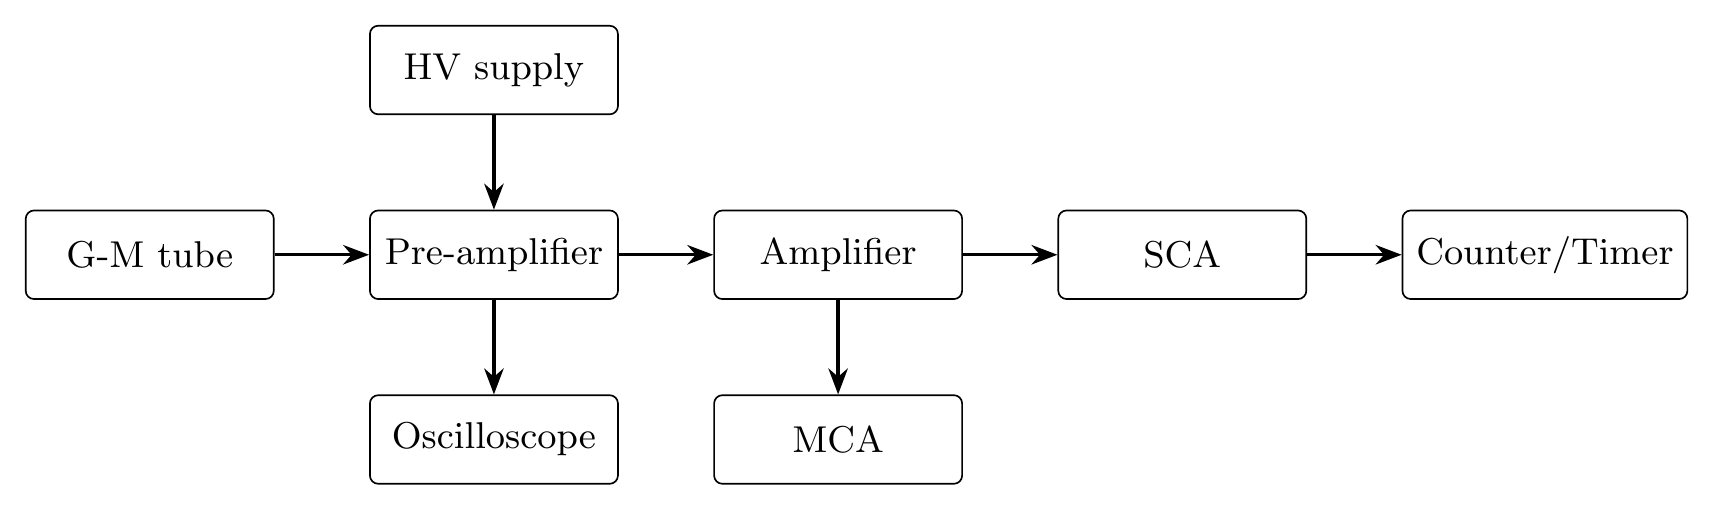
\includegraphics[width=0.5\linewidth]{block_diagram.png}
    \caption{Set-up diagram.}
    \label{fig:block}
\end{figure}


\subsection{Experimental Procedure}
\label{subsec:proced}



\section{Data}
\label{sec:data}
 
Count uncertainties are $\sigma_N = \sqrt{N}$ \cite{knoll}. All count times are Maestro live time, and we did not take a background count. The amplifier gain was 50 (coarse 100, fine 0.5) for the whole lab and the shaping time was 3~$\mu$s outside the shaping-time scan. No calculated result depends on the absolute gain, since it did not change during the lab.
 
We convert MCA channels to pulse amplitude with the calibration from our Lab 2 report, channel $= 765.8\,V + 27.6$, so
\begin{equation}
V = \frac{\text{channel} - 27.6}{765.8},
\label{eq:mcacal}
\end{equation}
with an amplitude uncertainty of 25.4~mV \cite{lab2}, the same conversion we used in Lab 4. This assumes the MCA was set up as in Lab 2. The three LLDs are channel 1738 ($2.23 \pm 0.03$~V, alpha), 307 ($0.36 \pm 0.03$~V, beta) and 229 ($0.26 \pm 0.03$~V, gamma).
 
\subsection{Shaping time}
 
Table~\ref{tab:rawshape} gives the Am-241 alpha peak centroid and gross area for each shaping time at 800~V, about 1 minute each. The centroid rises from 1723 at 0.5~$\mu$s to 2422 at 10~$\mu$s.
 
\begin{table}[!htbp]
\centering\small
\begin{tabular}{ccc}
\toprule
\textbf{Shaping time ($\mu$s)} & \textbf{Centroid (channel)} & \textbf{Gross area (counts)} \\
\midrule
0.5 & 1723.08 & 599257 $\pm$ 774 \\
1 & 2025.16 & 624639 $\pm$ 790 \\
2 & 2215.87 & 632332 $\pm$ 795 \\
3 & 2367.29 & 712298 $\pm$ 844 \\
6 & 2382.50 & 738092 $\pm$ 859 \\
10 & 2421.64 & 742365 $\pm$ 861 \\
\bottomrule
\end{tabular}
\caption{Alpha peak centroid and gross area vs shaping time, Am-241 at 800~V.}
\label{tab:rawshape}
\end{table}
 
\subsection{Alpha counting curve}
 
Table~\ref{tab:rawalpha} lists the gross counts above LLD channel 1738 (2.23~V) and the peak centroid, 30~s per point. We kept raising the voltage past the suggested 300--800~V \cite{labmanual} until the count rate leveled off. Counts first appeared at 400~V. At 1050~V the counts dropped from 669,674 to 286,105. We re-measured that point several times and got the same result, so we stopped there and took 1000~V as the start of the plateau. From 500 to 850~V the recorded centroid stays between 1744 and 2133, close to the LLD, and does not rise steadily.
 
\begin{table}[!htbp]
\centering\small\setlength{\tabcolsep}{3pt}
\begin{tabular}{ccc|ccc}
\toprule
\textbf{HV (V)} & \textbf{Counts (30 s)} & \textbf{Centroid} & \textbf{HV (V)} & \textbf{Counts (30 s)} & \textbf{Centroid} \\
\midrule
300 & 0 $\pm$ 0 & -- & 725 & 121059 $\pm$ 348 & 1753.07 \\
400 & 23 $\pm$ 5 & -- & 750 & 224018 $\pm$ 473 & 1881.92 \\
500 & 398 $\pm$ 20 & 1777.10 & 775 & 294972 $\pm$ 543 & 2118.21 \\
550 & 2516 $\pm$ 50 & 1764.00 & 800 & 390186 $\pm$ 625 & 1743.68 \\
600 & 11163 $\pm$ 106 & 1760.00 & 850 & 563218 $\pm$ 750 & 2133.17 \\
625 & 19972 $\pm$ 141 & 1765.85 & 900 & 617516 $\pm$ 786 & 2738.47 \\
650 & 32190 $\pm$ 179 & 1754.00 & 1000 & 669674 $\pm$ 818 & 3232.47 \\
675 & 46571 $\pm$ 216 & 1822.40 & 1050 & 286105 $\pm$ 535 & 7166.13 \\
700 & 61980 $\pm$ 249 & 1784.90 & & & \\
\bottomrule
\end{tabular}
\caption{Alpha counting curve, Am-241: gross counts above LLD channel 1738 (2.23~V) and peak centroid channel.}
\label{tab:rawalpha}
\end{table}
 
\subsection{Beta counting curve}
 
Table~\ref{tab:rawbeta} lists the Cl-36 counts above LLD channel 307 (0.36~V), 30~s per point. Counts first appeared at 1100~V and we stopped at 1550~V. The centroid stays near the LLD (305--335) up to 1450~V, then reads 508 and 773.
 
\begin{table}[!htbp]
\centering\small
\begin{tabular}{ccc}
\toprule
\textbf{HV (V)} & \textbf{Counts (30 s)} & \textbf{Centroid} \\
\midrule
1000 & 0 $\pm$ 0 & -- \\
1100 & 23161 $\pm$ 152 & 328.36 \\
1200 & 97809 $\pm$ 313 & 334.88 \\
1300 & 242325 $\pm$ 492 & 304.65 \\
1400 & 345372 $\pm$ 588 & 311.34 \\
1450 & 521827 $\pm$ 722 & 320.22 \\
1500 & 664725 $\pm$ 815 & 507.70 \\
1550 & 692883 $\pm$ 832 & 773.28 \\
\bottomrule
\end{tabular}
\caption{Beta counting curve, Cl-36: gross counts above LLD channel 307 (0.36~V) and centroid channel.}
\label{tab:rawbeta}
\end{table}
 
\subsection{Absolute efficiency}
 
We counted the Cl-36 source for 60~s at 1500~V, picked from the beta counting curve, with the same LLD (channel 307, 0.36~V) and gain: $1{,}428{,}191 \pm 1195$ counts. The source was marked 1.032~$\mu$Ci on August 1, 2026.
 
\subsection{Gamma response}
 
Table~\ref{tab:rawgamma} lists the counts with the Co-60 source turned upside down to block the betas, LLD channel 229 (0.26~V), 30~s per point. The counts rise to about 51,000 at 1500--1600~V and then fall at 1650 and 1700~V. We did not notice anything unusual at the time.
 
\begin{table}[!htbp]
\centering\small
\begin{tabular}{cc|cc}
\toprule
\textbf{HV (V)} & \textbf{Counts (30 s)} & \textbf{HV (V)} & \textbf{Counts (30 s)} \\
\midrule
1000 & 0 $\pm$ 0 & 1550 & 50648 $\pm$ 225 \\
1200 & 10490 $\pm$ 102 & 1600 & 51362 $\pm$ 227 \\
1300 & 24776 $\pm$ 157 & 1650 & 48634 $\pm$ 221 \\
1400 & 43711 $\pm$ 209 & 1700 & 43041 $\pm$ 207 \\
1500 & 51324 $\pm$ 227 & & \\
\bottomrule
\end{tabular}
\caption{Gamma response, Co-60 turned upside down: gross counts above LLD channel 229 (0.26~V).}
\label{tab:rawgamma}
\end{table}
 
\section{Analysis of Data}
\label{sec:analysis}
 
A rate from $N$ counts in time $t$ is $r = N/t$ with $\sigma_r = \sqrt{N}/t$ (Eq.~\ref{eq:th-rate}). Other uncertainties are propagated with Eq.~\ref{eq:th-prop}.
 
\subsection{Shaping time and ballistic deficit}
 
The ballistic deficit is the amplitude lost because the shaping time is too short to follow the whole pulse rise (Fig.~\ref{fig:th-bd}). Relative to 10~$\mu$s,
\begin{equation}
\text{BD} = \frac{C_{10} - C_{0.5}}{C_{10}} \times 100\%,
\end{equation}
with $C$ the centroid channel at each shaping time. The statistical uncertainty of a peak centroid is \cite{knoll}
\begin{equation}
\sigma_c = \frac{\text{FWHM}/2.35}{\sqrt{A}},
\end{equation}
with $A$ the peak area. We did not record the FWHM, so we cannot evaluate this. With $A \approx 6$--$7.4 \times 10^5$ counts, even a peak several hundred channels wide gives $\sigma_c$ below one channel, so we use $\sigma_c = 1$ channel as an upper bound. This only covers counting statistics, not the ROI placement or gain drift (Section~\ref{sec:amp}).
 
\begin{samplecalc}{Ballistic deficit at 0.5 $\mu$s ($C_{0.5} = 1723.08$, $C_{10} = 2421.64$, $\sigma_c = 1$)}
\begin{align*}
\text{BD} &= \frac{2421.64 - 1723.08}{2421.64} \times 100\% = 28.85\%\\
\sigma_{\text{BD}} &= 100\%\,\sigma_c\sqrt{\left(\frac{1}{C_{10}}\right)^2 + \left(\frac{C_{0.5}}{C_{10}^2}\right)^2}
 = 100\%\sqrt{(4.13\times10^{-4})^2 + (2.94\times10^{-4})^2} = 0.05\%
\end{align*}
\end{samplecalc}
 
\begin{figure}[!htbp]
\centering
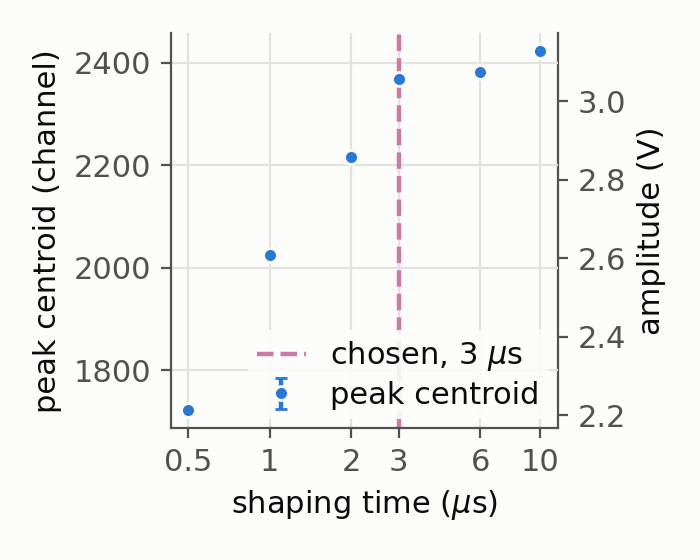
\includegraphics[width=0.55\textwidth]{F1_centroid_vs_shaping_time.png}
\caption{Alpha peak centroid vs shaping time at 800~V; right axis: amplitude from the Lab 2 calibration (Eq.~\ref{eq:mcacal}). Dashed line: chosen 3~$\mu$s. Error bars ($\pm$1 channel, upper bound) are smaller than the markers.}
\label{fig:shaping}
\end{figure}
 
The ballistic deficit at 0.5~$\mu$s relative to 10~$\mu$s is $28.85 \pm 0.05\%$. Figure~\ref{fig:shaping} shows the centroid climbing steeply up to 3~$\mu$s and then leveling off: the 3 and 6~$\mu$s centroids differ by only 15 channels. We chose 3~$\mu$s as the shortest shaping time without a significant deficit.
 
This follows from the pulse shape. Most of the signal comes from the positive ions drifting away from the anode wire. The pulse reaches half its height in about 0.25\% of the full ion collection time, but the full collection takes several hundred microseconds (Eqs.~\ref{eq:th-tion} and \ref{eq:th-thalf}). A shaping time of a few microseconds cuts off the slow remainder, and the shorter it is, the more amplitude is lost, so proportional counters need shaping times of several microseconds, long compared with the spread in pulse rise times \cite{knoll}. We did not measure the rise time of the amplifier output on the scope. A longer shaping time gives an output pulse that rises more slowly and peaks later, with an amplitude closer to the full value \cite{slides_shaping}.
 
\subsection{Alpha counting curve}
 
Table~\ref{tab:alpharate} gives the rates near the plateau (all rates are in Appendix~\ref{app:rates}) and Figure~\ref{fig:alphacc} shows the counting curve. We quote the plateau slope as the percent change in rate per 100~V, relative to the rate at the start of the range.
 
\begin{samplecalc}{Rate at 1000 V and plateau slope over 900--1000 V}
\begin{align*}
r_{1000} &= 669674/(30\ \text{s}) = 22322\ \text{s}^{-1}, & \sigma &= \sqrt{669674}/(30\ \text{s}) = 27\ \text{s}^{-1}\\
r_{900} &= 617516/(30\ \text{s}) = 20584\ \text{s}^{-1}, & \sigma &= \sqrt{617516}/(30\ \text{s}) = 26\ \text{s}^{-1}
\end{align*}
\begin{align*}
s_{\%} &= 100\,\frac{r_{1000} - r_{900}}{r_{900}} = 100\,\frac{1738.6}{20584} = 8.4\%\ \text{per 100 V},\\
\sigma_{s_\%} &= 100\,\frac{\sqrt{26^2 + 27^2}}{20584} = 0.2\%\ \text{per 100 V}
\end{align*}
\end{samplecalc}
 
\begin{figure}[!htbp]
\centering
\begin{minipage}[c]{0.36\textwidth}\centering\small
\begin{tabular}{cc}
\toprule
\textbf{HV (V)} & \textbf{Rate (s$^{-1}$)} \\
\midrule
850 & 18774 $\pm$ 25 \\
900 & 20584 $\pm$ 26 \\
1000 & 22322 $\pm$ 27 \\
1050 & 9537 $\pm$ 18 \\
\bottomrule
\end{tabular}
\captionof{table}{Alpha count rates near the plateau.}
\label{tab:alpharate}
\end{minipage}\hfill
\begin{minipage}[c]{0.60\textwidth}\centering
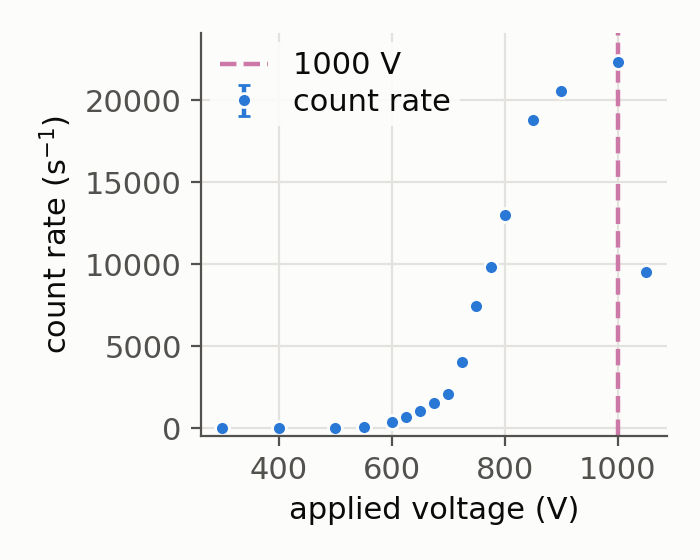
\includegraphics[width=\textwidth]{F2_alpha_counting_curve_lin.png}
\captionof{figure}{Alpha counting curve, Am-241, LLD channel 1738 (2.23~V); dashed line: 1000~V, start of the plateau. Error bars ($\sqrt{N}/t$) are smaller than the markers.}
\label{fig:alphacc}
\end{minipage}
\end{figure}
 
We expect no counts until the alpha pulses clear the LLD, a steep rise as the alpha peak crosses it, then a flat plateau once every alpha is counted (Fig.~\ref{fig:th-cc}). Ours has the rise, from 400 to 850~V, but flattens only over 900--1000~V, with a slope of 8.4~$\pm$~0.2\% per 100~V. So the plateau is barely established and not flat.
 
The drop to 9537~s$^{-1}$ at 1050~V is not expected. Past the plateau the rate should stay flat or climb as spurious pulses start to be counted \cite{knoll}. The counts were taken in live time, which corrects for the MCA dead time, so dead time is not the cause. Possible causes:
\begin{itemize}
\item amplifier saturation at high voltage \cite{labmanual}: the centroid at 1050~V is channel 7166, or 9.32~V by Eq.~\ref{eq:mcacal}, so a large part of the alpha peak sat at the top of the amplifier and MCA input range;
\item for the same reason, pulses above the top MCA channel are not recorded at all;
\item pile-up: at about $2\times10^4$~s$^{-1}$ with pulses several microseconds wide, the duty cycle (pulse width $\times$ rate) approaches $10^{-1}$, a high-rate situation \cite{knoll}, and live time does not correct for pile-up.
\end{itemize}
Saturation fits best, since the drop appears exactly where the peak reaches about 9~V. We left 1050~V out of the plateau and took 1000~V as its start. No later section uses the alpha operating point, so the drop does not affect the other results.
 
\textbf{Differential counting curve.} At a fixed LLD, the count rate vs voltage mirrors the integral pulse height distribution, so its slope maps the differential one (Fig.~\ref{fig:th-cc}) \cite{knoll}. We take the slope between neighbouring points, $dr/dV \approx (r_2 - r_1)/(V_2 - V_1)$, at the midpoint voltage, leaving out 1050~V.
 
\begin{samplecalc}{Slope between 725 and 750 V}
\begin{align*}
\frac{dr}{dV} &= \frac{7467.3 - 4035.3}{25\ \text{V}} = 137.3\ \text{s}^{-1}\text{V}^{-1}, &
\sigma &= \frac{\sqrt{15.8^2 + 11.6^2}}{25\ \text{V}} = 0.8\ \text{s}^{-1}\text{V}^{-1}
\end{align*}
\end{samplecalc}
 
\begin{figure}[!htbp]
\centering
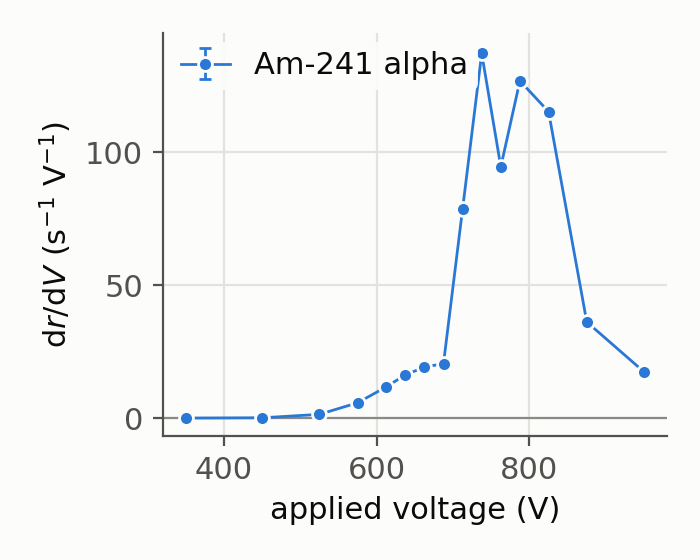
\includegraphics[width=0.55\textwidth]{F6a_alpha_differential.png}
\caption{Differential alpha counting curve, $dr/dV$ between neighbouring points of Figure~\ref{fig:alphacc}, plotted at the midpoint voltage. Higher voltage corresponds to smaller pulses. Error bars from Eq.~\ref{eq:th-prop}.}
\label{fig:alphadiff}
\end{figure}
 
Figure~\ref{fig:alphadiff} has three features. The main one is a single peak between 700 and 850~V, with its maximum near 740~V. This is the alpha peak sweeping past the LLD, and it holds most of the counts. The peak has a dip at 760~V that is far larger than its error bar. A small gain change between neighbouring points (Section~\ref{sec:amp}) is the likely cause. Before it, between 600 and 700~V, there is a smaller shoulder of about 20~s$^{-1}$~V$^{-1}$ that contains roughly 1700~s$^{-1}$, about 8\% of the plateau rate. These are pulses larger than the main peak and we cannot tell their origin without the spectrum. After the peak, the slope falls because of a tail of small pulses that only cross the LLD at the highest gains.
 
\subsection{Alpha pulse amplitude vs voltage}
\label{sec:amp}
 
The pulse charge is $Q = n_0 e M$ (Eq.~\ref{eq:th-charge}), and by the Diethorn model (Eq.~\ref{eq:th-diethorn}) $\ln M$ grows roughly linearly with $V$. So the centroid on a log axis vs voltage should follow a straight line, the trend of Fig.~\ref{fig:th-gain}. We compare neighbouring points with the two-point slope $s = \ln(C_2/C_1)/\Delta V$.
 
\begin{samplecalc}{Two-point slope, 900--1000 V ($C_1 = 2738.47$, $C_2 = 3232.47$, $\sigma_c = 1$)}
\begin{align*}
s &= \frac{\ln(3232.47/2738.47)}{100\ \text{V}} = 1.66\times10^{-3}\ \text{V}^{-1},\\
\sigma_s &= \frac{\sqrt{(1/2738.47)^2 + (1/3232.47)^2}}{100\ \text{V}} = 5\times10^{-6}\ \text{V}^{-1}
\end{align*}
The same for 1000--1050 V gives $s = (1.592 \pm 0.001)\times10^{-2}$ V$^{-1}$.
\end{samplecalc}
 
\begin{figure}[!htbp]
\centering
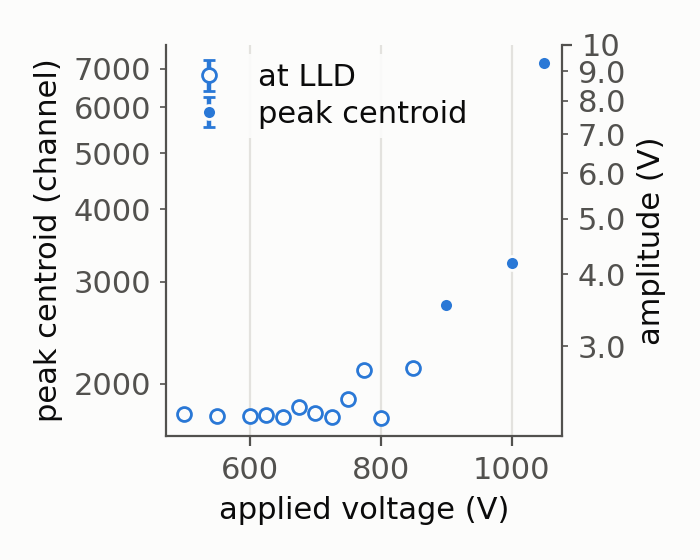
\includegraphics[width=0.55\textwidth]{F3_alpha_amplitude_vs_voltage_with_low.png}
\caption{Alpha peak centroid vs voltage on a log axis; right axis: amplitude from the Lab 2 calibration (Eq.~\ref{eq:mcacal}). Hollow: 500--850~V, where the centroid sits at the LLD. Error bars ($\pm$1 channel) are smaller than the markers.}
\label{fig:amp}
\end{figure}
 
From 500 to 850~V the centroid stays within a few hundred channels of the LLD (hollow points in Figure~\ref{fig:amp}). In this range the alpha peak was either below the LLD with only its upper edge counted, or not yet separated from the noise. Either way the number is the centroid of the counts above the LLD, not of the peak, so we leave these points out. This does not affect the counting curve, which only uses counts above the LLD; that range is where the alpha pulses cross the LLD.
 
That leaves 900, 1000 and 1050~V, and the 1050~V point is affected by saturation (previous section). The two slopes differ by about a factor of ten, so we cannot confirm the straight-line trend of Fig.~\ref{fig:th-gain} from our data. For scale, an example P-10 tube gains 17.4\% in $M$ for a 1\% increase in $V$ at 1793~V \cite{knoll}, or $\ln(1.174)/17.9\ \text{V} = 9\times10^{-3}$~V$^{-1}$, between our two values. Fig.~\ref{fig:th-gain} is for xenon mixtures, so only the trend compares.
 
The gas gain also changed between sections. In the shaping-time scan the peak sat at channel 2367 (3.06~V) at 800~V and 3~$\mu$s, but on the counting curve at the same voltage, amplifier gain and shaping time the centroid was at the LLD (2.23~V), and the 800~V count rate was only about 60\% of the plateau rate. Gas multiplication is very sensitive to small changes in high voltage and gas pressure \cite{knoll}, and we did not check a reference peak at the start of each section, so we cannot tell which one changed.
 
\subsection{Energy calibration}
 
We calibrate from the alpha peak centroid. Am-241 emits alphas at 5.486~MeV (85.2\%) and 5.443~MeV (12.8\%) \cite{knoll}, which our counter does not resolve, so we assign 5.486~MeV to the peak. With one peak, we assume the linear calibration passes through the origin, $E = k \times \text{channel}$. We use the 3~$\mu$s shaping-time run, where the ROI was drawn around the whole peak.
 
\begin{samplecalc}{Calibration factor (800 V, gain 50, 3 $\mu$s, $C = 2367.29$)}
\begin{align*}
k &= \frac{5486\ \text{keV}}{2367.29} = 2.317\ \text{keV/channel}, &
\sigma_k &= k\,\frac{\sigma_c}{C} = 2.317\,\frac{1}{2367.29} = 0.001\ \text{keV/channel}
\end{align*}
\end{samplecalc}
 
This factor holds only at 800~V, gain 50, 3~$\mu$s shaping, and the gas gain during the shaping-time runs. The same calculation at 1000~V on the counting curve would give 1.70~keV/channel. The differential counting curve (Figure~\ref{fig:alphadiff}) gives the shape of the pulse height distribution. It agrees with the expected one, a single alpha peak with noise and single-ion-pair events far below the LLD \cite{knoll}, apart from the small high-amplitude shoulder and the low-amplitude tail described above.
 
\subsection{Beta counting curve}
 
Figure~\ref{fig:bg} shows the Cl-36 beta counting curve with the gamma curve; the rates are in Appendix~\ref{app:rates}.
 
\begin{samplecalc}{Rate at 1500 V and plateau slope over 1500--1550 V}
\begin{align*}
r_{1500} &= 664725/(30\ \text{s}) = 22158\ \text{s}^{-1}, & \sigma &= 27\ \text{s}^{-1}\\
r_{1550} &= 692883/(30\ \text{s}) = 23096\ \text{s}^{-1}, & \sigma &= 28\ \text{s}^{-1}
\end{align*}
\begin{align*}
s_{\%} &= 100\,\frac{r_{1550} - r_{1500}}{r_{1500}}\cdot\frac{100\ \text{V}}{50\ \text{V}} = 8.5\%\ \text{per 100 V},\\
\sigma_{s_\%} &= 100\,\frac{\sqrt{27^2 + 28^2}}{22158}\cdot 2 = 0.4\%\ \text{per 100 V}
\end{align*}
\end{samplecalc}
 
\begin{figure}[!htbp]
\centering
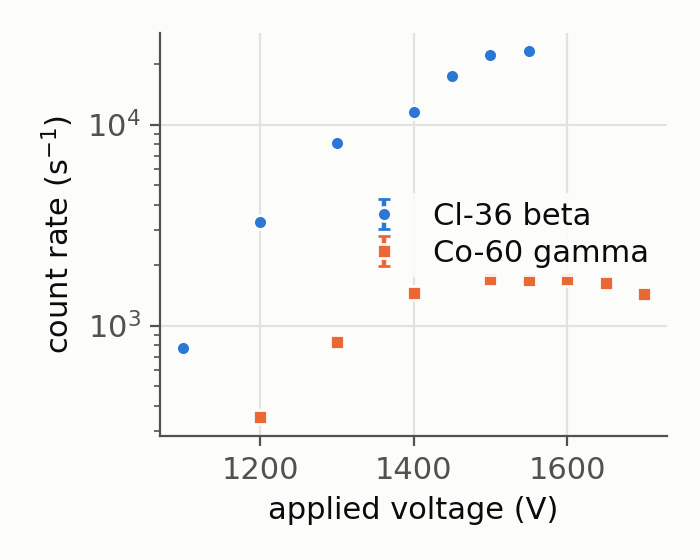
\includegraphics[width=0.55\textwidth]{F5_beta_gamma_counting_curves.png}
\caption{Counting curves for Cl-36 betas (LLD channel 307, 0.36~V) and Co-60 gammas (LLD channel 229, 0.26~V). Error bars ($\sqrt{N}/t$) are smaller than the markers.}
\label{fig:bg}
\end{figure}
 
We expect a beta counting curve that rises more gradually than the alpha curve and has a shorter, more sloped plateau, because the beta pulse heights are spread out and sit close to the noise (Fig.~\ref{fig:th-cc}). Ours rises over 1100--1500~V and flattens only between 1500 and 1550~V, with a slope of 8.5~$\pm$~0.4\% per 100~V.
 
The beta curve seems to have two plateaus, though the first is slight. The rate rises from 772 to 8078~s$^{-1}$ over 1100--1300~V, nearly levels off between 1300 and 1400~V, rises steeply again to 22158~s$^{-1}$ at 1500~V, and levels off a second time. The differential curve (Figure~\ref{fig:betadiff}, computed as for the alphas) shows this as two groups of pulses: a smaller peak near 1250~V and a larger one near 1425~V, with a dip at 1350~V.
 
\begin{figure}[!htbp]
\centering
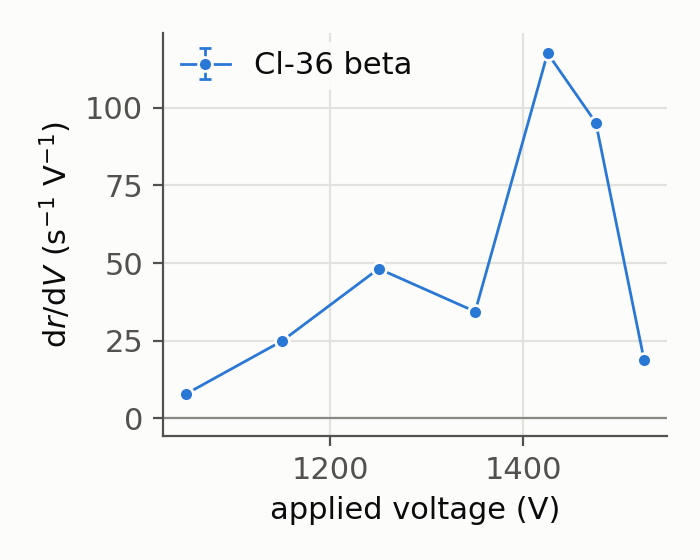
\includegraphics[width=0.55\textwidth]{F6b_beta_differential.png}
\caption{Differential Cl-36 counting curve, $dr/dV$ between neighbouring points of Figure~\ref{fig:bg}, plotted at the midpoint voltage. Error bars from Eq.~\ref{eq:th-prop}.}
\label{fig:betadiff}
\end{figure}
 
The shape looks like the counting curve of a mixed alpha and beta source, which has an alpha plateau followed by a beta plateau (Fig.~\ref{fig:th-cc}). It cannot be alphas here because Cl-36 is a pure beta emitter \cite{knoll}, and the curve has zero counts at 1000~V even though the LLD was only 0.36~V. On the alpha curve, alpha pulses were already above a 2.23~V LLD at 400--500~V, so any alpha would have been counted. The first plateau must therefore come from the largest beta pulses. A beta's pulse height depends on how much energy it leaves in the gas. Most Cl-36 betas cross the gas and reach the far wall, leaving only a small part of their energy. Low-energy betas, betas on long oblique paths, and betas backscattered from the source backing can leave much more \cite{knoll}. That splits the pulse heights into a smaller group of large pulses, counted first at 1100--1300~V, and the main group of small pulses, counted at 1400--1500~V. A gain change partway through the scan, like the one in Section~\ref{sec:amp}, could also produce a step, and without the spectrum we cannot rule it out.
 
The beta pulses are much smaller than the alpha pulses. At the same amplifier gain, alpha pulses cleared a 2.23~V LLD from 400--500~V, while beta pulses needed 1100~V to clear a 0.36~V LLD, and the beta centroid stayed at the LLD up to 1450~V. A beta's range is much longer than the chamber, so it loses only a small part of its energy in the gas, while an alpha stops in the gas and deposits all of it \cite{knoll}.
 
\subsection{Absolute and intrinsic efficiency}
 
The absolute efficiency is the number of pulses recorded per particle emitted, and the intrinsic efficiency is per particle that enters the detector. For an isotropic source they are related by the solid angle $\Omega$ (Eqs.~\ref{eq:th-eabs} and \ref{eq:th-eint}):
\begin{equation}
\varepsilon_{\text{abs}} = \frac{r}{A}, \qquad \varepsilon_{\text{int}} = \varepsilon_{\text{abs}}\,\frac{4\pi}{\Omega},
\end{equation}
with $\Omega = 2\pi$ for our counter. The activity on the day of the measurement is $A = A_0 e^{-\lambda t}$ with $\lambda = \ln 2/T_{1/2}$ (Eq.~\ref{eq:th-decay}) and $T_{1/2} = 3.08\times10^5$~y for Cl-36 \cite{knoll}, so the decay since August 1 is negligible. The marked activity has no stated uncertainty, so the quoted uncertainties are from counting only.
 
\begin{samplecalc}{Efficiency}
\begin{align*}
r &= 1428191/(60\ \text{s}) = 23803\ \text{s}^{-1}, & \sigma_r &= \sqrt{1428191}/(60\ \text{s}) = 20\ \text{s}^{-1}\\
A &= 1.032\ \mu\text{Ci} \times 3.7\times10^{4}\ \text{Bq}/\mu\text{Ci} = 38184\ \text{Bq} & &\\
\varepsilon_{\text{abs}} &= 23803/38184 = 0.6234, & \sigma &= 0.6234 \times 20/23803 = 0.0005\\
\varepsilon_{\text{int}} &= 0.6234 \times 4\pi/2\pi = 1.247, & \sigma &= 0.001
\end{align*}
\end{samplecalc}
 
\begin{table}[!htbp]
\centering\small
\begin{tabular}{lc}
\toprule
\textbf{Quantity} & \textbf{Value} \\
\midrule
Count rate $r$ (s$^{-1}$) & 23803 $\pm$ 20 \\
Activity $A$ (Bq) & 38184 \\
$\varepsilon_{\text{abs}}$ & 0.6234 $\pm$ 0.0005 \\
$\varepsilon_{\text{int}}$ ($\Omega = 2\pi$) & 1.247 $\pm$ 0.001 \\
\bottomrule
\end{tabular}
\caption{Absolute and intrinsic efficiency, Cl-36 at 1500~V (counting uncertainty only).}
\label{tab:eff}
\end{table}
 
For $2\pi$ geometry we expect an absolute efficiency of at most about 0.5 and an intrinsic efficiency for betas of about 100\% on the plateau, since every charged particle that enters the gas makes a pulse \cite{knoll}. We measured $\varepsilon_{\text{abs}} = 0.6234 \pm 0.0005$ and $\varepsilon_{\text{int}} = 1.247 \pm 0.001$ (Table~\ref{tab:eff}). An intrinsic efficiency above 100\% is not physical, so something added counts or the marked activity understates the source's beta output.
 
A likely cause is backscattering from the source backing. Betas emitted into the backing can scatter back out of the source surface and enter the counter, which raises the apparent yield \cite{knoll}. If a fraction $\eta$ of the betas emitted into the backing come back out, the absolute efficiency becomes $0.5(1+\eta)$, so our result needs $\eta = 2(0.6234) - 1 = 0.25$. Backscatter fractions of this size occur for electrons of a few hundred keV on medium-Z backings such as copper (Fig.~\ref{fig:th-backscatter}), so backscatter alone can explain the excess. Two smaller effects push the same way. The count rate was 7.4~$\pm$~0.2\% higher than on the beta counting curve at the same voltage, LLD and gain, which points to the same gain change as in Section~\ref{sec:amp}; on a short, sloped plateau, a higher gain brings in more small pulses. Spurious afterpulses also become more likely at high gas multiplication \cite{knoll}.
 
Background is not a likely cause. We did not take a background count, but in our previous labs the background was about 12~s$^{-1}$ \cite{lab3}.
 
\begin{samplecalc}{Background fraction (assumed $r_b \approx 12$ s$^{-1}$)}
\begin{align*}
\frac{r_b}{r} &= \frac{12}{23803} = 5\times10^{-4} = 0.05\%, &
\varepsilon_{\text{abs}} &= \frac{23803 - 12}{38184} = 0.6231
\end{align*}
\end{samplecalc}
 
Subtracting it would lower $\varepsilon_{\text{abs}}$ by only 0.0003, far too little to bring it below 0.5. Self-absorption in the source and a solid angle below $2\pi$ would lower the efficiency \cite{knoll}, so they cannot explain a value that is too high. To pin down the cause we should have taken a background count, checked the source certificate, repeated the measurement with the calibrated Am-241 alpha source, which avoids beta backscatter, and extended the beta counting curve past 1550~V so the operating point sits in the middle of a confirmed plateau rather than at its start.
 
\subsection{Gamma response}
 
\begin{samplecalc}{Gamma rate at 1500 V and plateau slope over 1500--1600 V}
\begin{align*}
r_{1500} &= 51324/(30\ \text{s}) = 1710.8\ \text{s}^{-1}, & \sigma &= \sqrt{51324}/(30\ \text{s}) = 7.6\ \text{s}^{-1}\\
s_{\%} &= 100\,\frac{1712.1 - 1710.8}{1710.8} = 0.1\%\ \text{per 100 V}, & \sigma_{s_\%} &= 100\,\frac{\sqrt{7.6^2 + 7.6^2}}{1710.8} = 0.6\%\ \text{per 100 V}
\end{align*}
\end{samplecalc}
 
We expect a gas counter to respond weakly to gamma rays. The chance of a gamma interacting in the gas falls quickly with energy (Fig.~\ref{fig:th-gammaabs}), and most counts come from interactions in the counter wall whose electrons reach the gas, with an intrinsic efficiency of only about a percent \cite{knoll}. Our Co-60 rate peaks at about 1710~s$^{-1}$, against about 22000~s$^{-1}$ for Cl-36 betas at the same voltage. Because those electrons lose different amounts of energy before reaching the gas, we expected a broad pulse-height spread and a gradual curve like the beta one. The curve in Figure~\ref{fig:bg} rises from 1200~V and is flat over 1500--1600~V (0.1~$\pm$~0.6\% per 100~V), then falls by 16\% by 1700~V. We did not notice anything at the time and the drop may come from the same saturation as the alpha drop.
 
 
\section{Conclusions}
\label{sec:conclusions}
 
The ballistic deficit at 0.5~$\mu$s relative to 10~$\mu$s was 28.85~$\pm$~0.05\%. The centroid levels off from 3~$\mu$s, so we chose 3~$\mu$s, as expected for the slow ion-drift tail of proportional counter pulses.
 
The alpha counting curve rose as expected but reached only a short, sloped plateau from 1000~V (8.4~$\pm$~0.2\% per 100~V), and the rate fell by more than half at 1050~V. The drop is most likely amplifier saturation, since the peak had reached 9.3~V. Next time we would lower the amplifier gain once the peak moves above about half of full scale, and watch the amplifier output on the scope at high voltage so a saturated peak is visible.
 
The alpha amplitude grew steeply with voltage, but the two usable slopes ($1.66\times10^{-3}$ and $1.59\times10^{-2}$~V$^{-1}$) differ by a factor of ten, so we could not confirm the expected straight line. The centroids below 900~V were cut off by the LLD, and the gas gain changed between sections. We would set the LLD lower for the amplitude measurement, record the peak centroid only once the whole peak is above it, and re-measure a reference peak at a fixed voltage at the start of each section to track the gain.
 
The energy calibration factor is 2.317~$\pm$~0.001~keV/channel at 800~V, gain 50 and 3~$\mu$s. The differential counting curve shows the expected single alpha peak, plus a small high-amplitude shoulder (about 8\% of counts) and a low-amplitude tail.
 
The beta counting curve had a short, sloped plateau (8.5~$\pm$~0.4\% per 100~V), and beta pulses were much smaller than alpha pulses, both as expected. It also had a slight first plateau at 1300--1400~V, which looks like an alpha plateau but cannot be one; we attribute it to a group of large beta pulses from betas that leave more energy in the gas. We would extend the scan past 1550~V, and take smaller voltage steps to resolve the two groups better.
 
The absolute efficiency was 0.6234~$\pm$~0.0005 and the intrinsic efficiency 1.247~$\pm$~0.001, above the 0.5 and 100\% limits. Backscattering from the source backing is the most likely cause, with the gain change adding a few percent; background is negligible (0.05\%). We would take a background count, check the source certificate and backing, and repeat with the Am-241 alpha source.
 
The Co-60 gamma rate peaked at 1712~$\pm$~8~s$^{-1}$, low as expected for a gas counter, with a flat region over 1500--1600~V and a 16\% drop by 1700~V that we did not expect. We would watch the amplifier output on the scope at high voltage to check for saturation.
 
\bibliography{references}
 
\appendix
\section{Count rates}
\label{app:rates}
 
\begin{table}[!htbp]
\centering\small\setlength{\tabcolsep}{4pt}
\begin{tabular}{cc|cc}
\toprule
\textbf{HV (V)} & \textbf{Rate (s$^{-1}$)} & \textbf{HV (V)} & \textbf{Rate (s$^{-1}$)} \\
\midrule
300 & 0.00 $\pm$ 0.00 & 725 & 4035.3 $\pm$ 11.6 \\
400 & 0.77 $\pm$ 0.16 & 750 & 7467.3 $\pm$ 15.8 \\
500 & 13.27 $\pm$ 0.66 & 775 & 9832.4 $\pm$ 18.1 \\
550 & 83.9 $\pm$ 1.7 & 800 & 13006.2 $\pm$ 20.8 \\
600 & 372.1 $\pm$ 3.5 & 850 & 18773.9 $\pm$ 25.0 \\
625 & 665.7 $\pm$ 4.7 & 900 & 20583.9 $\pm$ 26.2 \\
650 & 1073.0 $\pm$ 6.0 & 1000 & 22322.5 $\pm$ 27.3 \\
675 & 1552.4 $\pm$ 7.2 & 1050 & 9536.8 $\pm$ 17.8 \\
700 & 2066.0 $\pm$ 8.3 & & \\
\bottomrule
\end{tabular}
\caption{Alpha count rates, $r = N/30$~s, $\sigma_r = \sqrt{N}/30$~s.}
\label{tab:appalpha}
\end{table}
 
\begin{table}[!htbp]
\centering\small
\begin{tabular}{ccc}
\toprule
\textbf{HV (V)} & \textbf{Cl-36 beta (s$^{-1}$)} & \textbf{Co-60 gamma (s$^{-1}$)} \\
\midrule
1000 & 0.0 $\pm$ 0.0 & 0.0 $\pm$ 0.0 \\
1100 & 772.0 $\pm$ 5.1 & -- \\
1200 & 3260.3 $\pm$ 10.4 & 349.7 $\pm$ 3.4 \\
1300 & 8077.5 $\pm$ 16.4 & 825.9 $\pm$ 5.2 \\
1400 & 11512.4 $\pm$ 19.6 & 1457.0 $\pm$ 7.0 \\
1450 & 17394.2 $\pm$ 24.1 & -- \\
1500 & 22157.5 $\pm$ 27.2 & 1710.8 $\pm$ 7.6 \\
1550 & 23096.1 $\pm$ 27.7 & 1688.3 $\pm$ 7.5 \\
1600 & -- & 1712.1 $\pm$ 7.6 \\
1650 & -- & 1621.1 $\pm$ 7.4 \\
1700 & -- & 1434.7 $\pm$ 6.9 \\
\bottomrule
\end{tabular}
\caption{Beta and gamma count rates, $r = N/30$~s, $\sigma_r = \sqrt{N}/30$~s.}
\label{tab:appbg}
\end{table}
 
\end{document}
